% SPDX-License-Identifier: CC-BY-SA-4.0
%
% Copyright (c) 2020 Philipp Le
%
% Except where otherwise noted, this work is licensed under a
% Creative Commons Attribution-ShareAlike 4.0 License.
%
% Please find the full copy of the licence at:
% https://creativecommons.org/licenses/by-sa/4.0/legalcode

\chapter{Modulation and Mixing}

\begin{refsection}
	
The task of a communication system is transmitting information.

Example: Voice transmission
\begin{itemize}
	\item Voice has a spectrum from about \SI{20}{Hz} to \SI{20}{kHz}
	\item It is not feasible to transmit the spectrum directly as electromagnetic waves.
	\item The electromagnetic spectrum must be shared with myriads of other users.
	\item So, the voice is shifted to a higher frequency, for example, \SI{144.3}{MHz}.
	\item The voice is \emph{modulated} on this \emph{carrier} of \SI{144.3}{MHz}.
	\item The voice is then located from about \SI{144.28}{MHz} to \SI{144.32}{MHz}.
\end{itemize}

\begin{definition}{Modulation}
	\index{modulation} \textbf{Modulation} is the process of altering a signal -- the \index{carrier} \textbf{carrier} -- so that it contains the information to be transmitted.
\end{definition}

\begin{definition}{Demodulation}
	\index{demodulation} \textbf{Demodulation} is the inverse process of modulation. The information is extracted from the carrier.
\end{definition}

In the previous example, the voice was the information-carrying signal. This can be transferred to any kind of information. In this chapter, we will discuss techniques to modulate data on carriers which can be transmitted over wired and wireless channels.

\todo{Block diagram modulator}

\section{Modulation in The Time and Frequency Domain}

Generally, the carrier is a \emph{monochromatic} signal, i.e., it is a sinusoidal function. A sinusoidal function has three parameters: (angular) frequency $\omega_C$, phase $\varphi_C$ and amplitude $\hat{X}_C$.
\begin{equation}
	x_C(t) = \hat{X}_C \cos\left(\omega_C t + \varphi_C\right)
	\label{eq:ch05:carrier_timedomain}
\end{equation}
The frequency is fixed to the carrier frequency. The other two parameters can be altered and the information can be modulated into them.

There are two classes of modulation:
\begin{itemize}
	\item \textbf{Amplitude modulation} The amplitude of the carrier is altered.
	\begin{equation}
		x_{S,AM}(t) = f_{\hat{X}}(t) \cos\left(\omega_C t + \varphi_C\right)
	\end{equation}
	\item \textbf{Phase modulation} The phase of the carrier is altered.
	\begin{equation}
		x_{S,PM}(t) = \hat{X}_C \cos\left(\omega_C t + f_{\varphi}(t)\right)
	\end{equation}
\end{itemize}

This section covers basic modulation techniques of analogue signals.
\begin{itemize}
	\item The considerations are explanatory and are extended to digital signals in the following section.
	\item This section shall offer an understanding of how modulation works in general (for both analogue and digital signals).
	\item A digital signal must be converted to an analogue signal in order to physically exists. It can then be modulated onto a carrier and transmitted as an electromagnetic wave.
\end{itemize}

\subsection{Amplitude Modulation}

The \index{amplitude modulation} \textbf{\ac{AM}} is the alteration of the carrier's amplitude.

\begin{attention}
	By now, all signals are real, because the technical realization is considered. Physical signals must always be real.
\end{attention}

The carrier is a mono-chromatic signal:
\begin{equation}
	x_C(t) = \hat{X}_C \cdot \cos\left(2\pi f_C + \varphi_C\right)
\end{equation}
where
\begin{itemize}
	\item $\hat{X}_C$ is the amplitude of the carrier,
	\item $f_C$ is the carrier frequency ($2\pi f_C = \omega_C$ is carrier angular frequency), and
	\item $\varphi_C$ is the phase offset of the carrier.
\end{itemize}

The carrier amplitude can be altered by multiplying it with the instantaneous value of the information-carrying signal $x_B(t)$:
\begin{equation}
	x_{DSB-TC}(t) = x_B(t) \cdot \left(1 + \mu x_C(t)\right)
	\label{eq:ch05:amdsb_timedomain}
\end{equation}
\begin{itemize}
	\item The waveform of the carrier is retained. The carrier is still present in the modulated signal. This is represented by the $+1$ in the sum.
	\item Its amplitude is changed by the instantaneous value of the information-carrying signal. The contribution of the information-carrying signal is defined by the factor $\mu$.
\end{itemize}

\begin{figure}[H]
	\centering
	
	\subfloat[Carrier and information-carrying signals]{
		\centering
		\begin{tikzpicture}
			\begin{axis}[
				height={0.15\textheight},
				width=0.6\linewidth,
				scale only axis,
				xlabel={$t$},
				ylabel={$x(t)$},
				%grid style={line width=.6pt, color=lightgray},
				%grid=both,
				grid=none,
				legend pos=outer north east,
				axis y line=middle,
				axis x line=middle,
				every axis x label/.style={
					at={(ticklabel* cs:1.05)},
					anchor=north,
				},
				every axis y label/.style={
					at={(ticklabel* cs:1.05)},
					anchor=east,
				},
				xmin=-0.5,
				xmax=8.5,
				ymin=-1.2,
				ymax=1.2,
				%xtick={0,0.125,...,1},
				%xticklabels={$- \omega_S$, $- \frac{\omega_S}{2}$, $0$, $\frac{\omega_S}{2}$, $\omega_S$},
				%ytick={0},
			]
				\addplot[blue, smooth, domain=0:8, samples=200] plot(\x, {cos(deg(2*pi*2*\x))});
				\addlegendentry{Carrier $x_C(t)$};
				\addplot[red, smooth, domain=0:8, samples=50] plot(\x, {cos(deg(2*pi*0.25*\x))});
				\addlegendentry{Information $x_B(t)$};
			\end{axis}
		\end{tikzpicture}
	}

	\subfloat[\acs{DSB-TC} \acs{AM} (with carrier)]{
		\centering
		\begin{tikzpicture}
			\begin{axis}[
				height={0.15\textheight},
				width=0.6\linewidth,
				scale only axis,
				xlabel={$t$},
				ylabel={$x_{DSB-TC}(t)$},
				%grid style={line width=.6pt, color=lightgray},
				%grid=both,
				grid=none,
				legend pos=outer north east,
				axis y line=middle,
				axis x line=middle,
				every axis x label/.style={
					at={(ticklabel* cs:1.05)},
					anchor=north,
				},
				every axis y label/.style={
					at={(ticklabel* cs:1.05)},
					anchor=east,
				},
				xmin=-0.5,
				xmax=8.5,
				ymin=-1.7,
				ymax=1.7,
				%xtick={0,0.125,...,1},
				%xticklabels={$- \omega_S$, $- \frac{\omega_S}{2}$, $0$, $\frac{\omega_S}{2}$, $\omega_S$},
				%ytick={0},
			]
				\addplot[red, smooth, domain=0:8, samples=150] plot(\x, {cos(deg(2*pi*2*\x)) * (1+0.5*cos(deg(2*pi*0.25*\x)))});
				\addlegendentry{\acs{DSB} Signal $x_{DSB-TC}(t)$};
				\addplot[olive, dashed, smooth, domain=0:8, samples=150] plot(\x, {(1+0.5*cos(deg(2*pi*0.25*\x)))});
				\addlegendentry{Envelope of $x_B(t)$};
			\end{axis}
		\end{tikzpicture}
	}

	\caption{\acs{DSB} \acs{AM} of analogue signals}
\end{figure}

\subsubsection{Frequency Domain}

Assumptions for the information-carrying signal:
\begin{itemize}
	\item The information-carrying signal is band-limited to $-f_B \geq f \geq f_B$ ($\underline{X}_B\left(j\omega\right) = 0 \quad \forall \; |f| > f_B$).
	\item The information-carrying signal is real-valued. Its spectrum is therefore symmetric ($\underline{X}_B\left(j\omega\right) = \overline{\underline{X}_B\left(-j\omega\right)}$).
\end{itemize}

The carrier is monochromatic \eqref{eq:ch05:carrier_timedomain}. Its \ac{CTFT} is:
\begin{equation}
	\underline{X}_C\left(j\omega\right) = \hat{X}_C \pi \left( \delta\left(\omega + 2 \pi f_C \right) + \delta\left(\omega - 2 \pi f_C \right) \right)
\end{equation}

The time-domain expression \eqref{eq:ch05:amdsb_timedomain} of the \ac{AM} is in the frequency domain:
\begin{equation}
	\underline{X}_{DSB-TC}\left(j\omega\right) = \underline{X}_C\left(j\omega\right) + \mu \underline{X}_C\left(j\omega\right) * \underline{X}_B\left(j\omega\right)
\end{equation}
The multiplication becomes a convolution.
\begin{equation}
	\underline{X}_{DSB-TC}\left(j\omega\right) = \hat{X}_C \pi \left( \underbrace{\delta\left(\omega + 2 \pi f_C \right) + \mu \underline{X}_B\left(j\left(\omega + 2 \pi f_C\right)\right)}_{\text{Carrier plus frequency-shifted information (-)}} + \underbrace{\delta\left(\omega - 2 \pi f_C \right) + \mu \underline{X}_B\left(j\left(\omega - 2 \pi f_C\right)\right)}_{\text{Carrier plus frequency-shifted information (+)}} \right)
\end{equation}

\textbf{The \ac{AM} is a frequency shift of the information-carrying in both the positive and the negative direction.}

Due to the symmetry of the information-carrying signal, there is an \emph{upper sideband} and a \emph{lower sideband}, carrying the identical information, around the carrier.

Because of the presence of the carrier and both sidebands, the modulation is called \index{double-sideband!transmitted carrier} \textbf{\acf{DSB-TC}}.

\begin{definition}{Transmission bandwidth of \acs{DSB} \acs{AM}}
	The modulated signal of the \acs{DSB} \acs{AM} consists of the positive and negative part of the information-carrying signal shifted in frequency to the carrier frequency. The information-carrying signal emerges as sidebands.
	
	Therefore, the bandwidth of the modulated signal is $[\omega_C - \omega_B, \omega_C + \omega_B]$. The difference $2 \omega_B$ is called \index{transmission bandwidth} \textbf{transmission bandwidth}.
\end{definition}

\begin{fact}
	The transmission bandwidth of \acs{DSB} \acs{AM} is the double of the maximum frequency in the information-carrying signal $2 \omega_B$.
\end{fact}

\begin{figure}[H]
	\subfloat[Information-carrying signal $\underline{X}_B\left(j\omega\right)$ (real-valued in time-domain)] {
		\centering
		\begin{tikzpicture}
			\begin{axis}[
				height={0.15\textheight},
				width=0.9\linewidth,
				scale only axis,
				xlabel={$\omega$},
				ylabel={$|\underline{X}_B\left(j\omega\right)|$},
				%grid style={line width=.6pt, color=lightgray},
				%grid=both,
				grid=none,
				legend pos=north east,
				axis y line=middle,
				axis x line=middle,
				every axis x label/.style={
					at={(ticklabel* cs:1.05)},
					anchor=north,
				},
				every axis y label/.style={
					at={(ticklabel* cs:1.05)},
					anchor=east,
				},
				xmin=-3.5,
				xmax=3.5,
				ymin=0,
				ymax=1.2,
				xtick={-0.5, 0, 0.5},
				xticklabels={$- \omega_B$, $0$, $\omega_B$},
				ytick={0},
			]
				\draw[red, thick] (axis cs:-0.5,0) -- (axis cs:0,0.7);
				\draw[red, thick] (axis cs:0,0.7) -- (axis cs:0.5,0);
			\end{axis}
		\end{tikzpicture}
	}
	
	\subfloat[Carrier signal $\underline{X}_C\left(j\omega\right)$ (real-valued in time-domain)] {
		\centering
		\begin{tikzpicture}
			\begin{axis}[
				height={0.15\textheight},
				width=0.9\linewidth,
				scale only axis,
				xlabel={$\omega$},
				ylabel={$|\underline{X}_C\left(j\omega\right)|$},
				%grid style={line width=.6pt, color=lightgray},
				%grid=both,
				grid=none,
				legend pos=north east,
				axis y line=middle,
				axis x line=middle,
				every axis x label/.style={
					at={(ticklabel* cs:1.05)},
					anchor=north,
				},
				every axis y label/.style={
					at={(ticklabel* cs:1.05)},
					anchor=east,
				},
				xmin=-3.5,
				xmax=3.5,
				ymin=0,
				ymax=1.2,
				xtick={-2, 0, 2},
				xticklabels={$- \omega_C$, $0$, $\omega_C$},
				ytick={0},
			]
				\pgfplotsinvokeforeach{-2, 2}{
					\draw[-latex, blue, very thick] (axis cs:#1,0) -- (axis cs:#1,1);
				}
			\end{axis}
		\end{tikzpicture}
	}
	
	\subfloat[\acs{AM} \acs{DSB-TC} modulated signal $\underline{X}_{DSB-TC}\left(j\omega\right)$ with frequency-shifted information and carrier (real-valued in time-domain)] {
		\centering
		\begin{tikzpicture}
			\begin{axis}[
				height={0.15\textheight},
				width=0.9\linewidth,
				scale only axis,
				xlabel={$\omega$},
				ylabel={$|\underline{X}_{DSB-TC}\left(j\omega\right)|$},
				%grid style={line width=.6pt, color=lightgray},
				%grid=both,
				grid=none,
				legend pos=north east,
				axis y line=middle,
				axis x line=middle,
				every axis x label/.style={
					at={(ticklabel* cs:1.05)},
					anchor=north,
				},
				every axis y label/.style={
					at={(ticklabel* cs:1.05)},
					anchor=east,
				},
				xmin=-3.5,
				xmax=3.5,
				ymin=0,
				ymax=1.2,
				xtick={-2, 0, 2},
				xticklabels={$- \omega_C$, $0$, $\omega_C$},
				ytick={0},
			]
				\pgfplotsinvokeforeach{-2, 2}{
					\draw[-latex, red, very thick] (axis cs:#1,0) -- (axis cs:#1,1);
					\draw[red, thick] (axis cs:{#1-0.5},0) -- (axis cs:#1,0.7);
					\draw[red, thick] (axis cs:#1,0.7) -- (axis cs:{#1+0.5},0);
				}
			\end{axis}
		\end{tikzpicture}
	}
	
	\caption{Spectrum of the \acs{DSB-TC} \acs{AM} signal}
\end{figure}

\subsection{Carrier Suppression}

The carrier does not contain any information. It can therefore be removed from the modulated signal. The $+1$ of \eqref{eq:ch05:amdsb_timedomain} is dropped. The \ac{AM} becomes a simple multiplication.
\begin{equation}
	x_{DSB-SC}(t) = x_B(t) \cdot x_C(t)
	\label{eq:ch05:amdsbsc_timedomain}
\end{equation}

\begin{figure}[H]
	\centering
	
	\subfloat[Carrier and information-carrying signals]{
		\centering
		\begin{tikzpicture}
			\begin{axis}[
				height={0.15\textheight},
				width=0.6\linewidth,
				scale only axis,
				xlabel={$t$},
				ylabel={$x(t)$},
				%grid style={line width=.6pt, color=lightgray},
				%grid=both,
				grid=none,
				legend pos=outer north east,
				axis y line=middle,
				axis x line=middle,
				every axis x label/.style={
					at={(ticklabel* cs:1.05)},
					anchor=north,
				},
				every axis y label/.style={
					at={(ticklabel* cs:1.05)},
					anchor=east,
				},
				xmin=-0.5,
				xmax=8.5,
				ymin=-1.2,
				ymax=1.2,
				%xtick={0,0.125,...,1},
				%xticklabels={$- \omega_S$, $- \frac{\omega_S}{2}$, $0$, $\frac{\omega_S}{2}$, $\omega_S$},
				%ytick={0},
			]
				\addplot[blue, smooth, domain=0:8, samples=200] plot(\x, {cos(deg(2*pi*2*\x))});
				\addlegendentry{Carrier $x_C(t)$};
				\addplot[red, smooth, domain=0:8, samples=50] plot(\x, {cos(deg(2*pi*0.25*\x))});
				\addlegendentry{Information $x_B(t)$};
			\end{axis}
		\end{tikzpicture}
	}
	
	\subfloat[\acs{DSB-SC} \acs{AM} (carrier suppressed)]{
		\centering
		\begin{tikzpicture}
			\begin{axis}[
				height={0.15\textheight},
				width=0.6\linewidth,
				scale only axis,
				xlabel={$t$},
				ylabel={$x_{DSB-SC}(t)$},
				%grid style={line width=.6pt, color=lightgray},
				%grid=both,
				grid=none,
				legend pos=outer north east,
				axis y line=middle,
				axis x line=middle,
				every axis x label/.style={
					at={(ticklabel* cs:1.05)},
					anchor=north,
				},
				every axis y label/.style={
					at={(ticklabel* cs:1.05)},
					anchor=east,
				},
				xmin=-0.5,
				xmax=8.5,
				ymin=-1.2,
				ymax=1.2,
				%xtick={0,0.125,...,1},
				%xticklabels={$- \omega_S$, $- \frac{\omega_S}{2}$, $0$, $\frac{\omega_S}{2}$, $\omega_S$},
				%ytick={0},
			]
				\addplot[red, smooth, domain=0:8, samples=150] plot(\x, {cos(deg(2*pi*2*\x)) * (cos(deg(2*pi*0.25*\x)))});
				\addlegendentry{\acs{DSB-SC} Signal $x_{DSB-SC}(t)$};
				\addplot[olive, dashed, smooth, domain=0:8, samples=150] plot(\x, {(cos(deg(2*pi*0.25*\x)))});
				\addlegendentry{Envelope of $x_B(t)$};
			\end{axis}
		\end{tikzpicture}
	}
	
	\caption{\acs{DSB-SC} \acs{AM} of analogue signals}
\end{figure}

The multiplication in the time-domain becomes a convolution in the frequency domain:
\begin{equation}
	\begin{split}
		\underline{X}_{DSB-SC}\left(j\omega\right) &= \underline{X}_C\left(j\omega\right) * \underline{X}_B\left(j\omega\right) \\
		 &= \hat{X}_C \pi \left( \underbrace{\underline{X}_B\left(j\left(\omega + 2 \pi f_C\right)\right)}_{\text{Frequency-shifted information (-)}} + \underbrace{\underline{X}_B\left(j\left(\omega - 2 \pi f_C\right)\right)}_{\text{Frequency-shifted information (+)}} \right)
	\end{split}
\end{equation}

The information-carrying signal is frequency-shifted in both positive and negative directions. It emerges as two sidebands at carrier frequency. However, the carrier is not present in the output signal. Therefore, the modulation is called \index{double-sideband!suppressed carrier} \textbf{\acf{DSB-SC}}.

Like the \ac{DSB-TC}, the transmission bandwidth of the \ac{DSB-SC} is $2 \omega_B$.

\begin{figure}[H]
	\subfloat[Information-carrying signal $\underline{X}_B\left(j\omega\right)$ (real-valued in time-domain)] {
		\centering
		\begin{tikzpicture}
			\begin{axis}[
				height={0.15\textheight},
				width=0.9\linewidth,
				scale only axis,
				xlabel={$\omega$},
				ylabel={$|\underline{X}_B\left(j\omega\right)|$},
				%grid style={line width=.6pt, color=lightgray},
				%grid=both,
				grid=none,
				legend pos=north east,
				axis y line=middle,
				axis x line=middle,
				every axis x label/.style={
					at={(ticklabel* cs:1.05)},
					anchor=north,
				},
				every axis y label/.style={
					at={(ticklabel* cs:1.05)},
					anchor=east,
				},
				xmin=-3.5,
				xmax=3.5,
				ymin=0,
				ymax=1.2,
				xtick={-0.5, 0, 0.5},
				xticklabels={$- \omega_B$, $0$, $\omega_B$},
				ytick={0},
			]
				\draw[red, thick] (axis cs:-0.5,0) -- (axis cs:0,0.7);
				\draw[red, thick] (axis cs:0,0.7) -- (axis cs:0.5,0);
			\end{axis}
		\end{tikzpicture}
	}
	
	\subfloat[Carrier signal $\underline{X}_C\left(j\omega\right)$ (real-valued in time-domain)] {
		\centering
		\begin{tikzpicture}
			\begin{axis}[
				height={0.15\textheight},
				width=0.9\linewidth,
				scale only axis,
				xlabel={$\omega$},
				ylabel={$|\underline{X}_C\left(j\omega\right)|$},
				%grid style={line width=.6pt, color=lightgray},
				%grid=both,
				grid=none,
				legend pos=north east,
				axis y line=middle,
				axis x line=middle,
				every axis x label/.style={
					at={(ticklabel* cs:1.05)},
					anchor=north,
				},
				every axis y label/.style={
					at={(ticklabel* cs:1.05)},
					anchor=east,
				},
				xmin=-3.5,
				xmax=3.5,
				ymin=0,
				ymax=1.2,
				xtick={-2, 0, 2},
				xticklabels={$- \omega_C$, $0$, $\omega_C$},
				ytick={0},
			]
				\pgfplotsinvokeforeach{-2, 2}{
					\draw[-latex, blue, very thick] (axis cs:#1,0) -- (axis cs:#1,1);
				}
			\end{axis}
		\end{tikzpicture}
	}
	
	\subfloat[\acs{AM} \acs{DSB} modulated signal $\underline{X}_{DSB}\left(j\omega\right)$ with frequency-shifted information (real-valued in time-domain). The carrier is suppressed.] {
		\centering
		\begin{tikzpicture}
			\begin{axis}[
				height={0.15\textheight},
				width=0.9\linewidth,
				scale only axis,
				xlabel={$\omega$},
				ylabel={$|\underline{X}_{DSB}\left(j\omega\right)|$},
				%grid style={line width=.6pt, color=lightgray},
				%grid=both,
				grid=none,
				legend pos=north east,
				axis y line=middle,
				axis x line=middle,
				every axis x label/.style={
					at={(ticklabel* cs:1.05)},
					anchor=north,
				},
				every axis y label/.style={
					at={(ticklabel* cs:1.05)},
					anchor=east,
				},
				xmin=-3.5,
				xmax=3.5,
				ymin=0,
				ymax=1.2,
				xtick={-2, 0, 2},
				xticklabels={$- \omega_C$, $0$, $\omega_C$},
				ytick={0},
			]
				\pgfplotsinvokeforeach{-2, 2}{
					\draw[red, thick] (axis cs:{#1-0.5},0) -- (axis cs:#1,0.7);
					\draw[red, thick] (axis cs:#1,0.7) -- (axis cs:{#1+0.5},0);
				}
			\end{axis}
		\end{tikzpicture}
	}
	
	\caption{Spectrum of the \acs{DSB-SC} \acs{AM} signal}
\end{figure}

\subsubsection{Sideband suppression}

\begin{itemize}
	\item The two sidebands contain identical information.
	\item Therefore, one sideband can be removed without losing information.
	\item High-quality filters with steep slopes in the amplitude response may be used to suppress one the side bands.
	\item The resulting \index{single-sideband} \textbf{\ac{SSB} \ac{AM}} is mainly used for analogue signals, which is out of the scope of this lecture.
\end{itemize}

\subsection{Phase Modulation}

\todo{Phase Modulation}

\section{Frequency mixer}

The information-carrying signal and the carrier are usually at different frequencies. A communication system must therefore be able to shift between multiple frequencies. Such communication systems are called \index{heterodyne} \textbf{heterodyne}.

\begin{itemize}
	\item The modulation and demodulation happen at a low, near-zero frequency. The modulated signal is the \index{baseband signal} \textbf{baseband signal}.
	\item A device called \index{mixer} \textbf{mixer} converts one frequency to another. The modulated information is kept intact.
\end{itemize}

\begin{figure}[H]
	\centering
	
	\subfloat[Heterodyne transmitter without \acs{IF} stage]{
		\centering
		\begin{adjustbox}{scale=0.8}
			\begin{circuitikz}
				\node[block, draw](Baseband){Baseband\\ modulation};
				\node[mixer, right=2.5cm of Baseband](Mixer){};
				\node[ampshape, right=4cm of Mixer](Amplifier){};
				
				\draw (Mixer.south) node[below,align=center,yshift=-5mm]{Mixer};
				\draw (Amplifier.south) node[below,align=center,yshift=-5mm]{\acs{RF}\\ amplifier};
				
				\draw[-latex] (Baseband.east) -- node[midway,above,align=center]{Baseband\\ signal} (Mixer.west);
				\draw[-latex] (Mixer.east) to[bandpass] ++(2cm,0) -- node[midway,above,align=center]{\acs{RF}\\ signal} (Amplifier.west);
				\draw (Amplifier.east) to[bandpass] ++(2cm,0) -- ++(0,0) node[txantenna]{};
			\end{circuitikz}
		\end{adjustbox}
	}

	\subfloat[Heterodyne receiver without \acs{IF} stage]{
		\centering
		\begin{adjustbox}{scale=0.8}
			\begin{circuitikz}
				\node[ampshape](RFAmplifier){};
				\node[mixer, right=2cm of RFAmplifier](Mixer){};
				\node[ampshape, right=2.5cm of Mixer](BBAmplifier){};
				\node[block, draw, right=2.5cm of BBAmplifier](Baseband){Baseband\\ demodulation};
				
				\draw (RFAmplifier.south) node[below,align=center,yshift=-5mm]{\acs{RF}\\ amplifier};
				\draw (Mixer.south) node[below,align=center,yshift=-5mm]{Mixer};
				\draw (BBAmplifier.south) node[below,align=center,yshift=-5mm]{Baseband\\ amplifier};
				
				\draw (RFAmplifier.west) to[bandpass] ++(-2cm,0) node[rxantenna,xscale=-1]{};
				
				\draw[-latex] (RFAmplifier.east) -- node[midway,above,align=center]{\acs{RF}\\ signal} (Mixer.west);
				\draw[-latex] (Mixer.east) to[bandpass] ++(2cm,0) -- (BBAmplifier.west);
				\draw[-latex] (BBAmplifier.east) -- node[midway,above,align=center]{Baseband\\ signal} (Baseband.west);
			\end{circuitikz}
		\end{adjustbox}
	}

	\subfloat[Superheterodyne receiver]{
		\centering
		\begin{adjustbox}{scale=0.6}
			\begin{circuitikz}
				\node[ampshape](RFAmplifier){};
				\node[mixer, right=2cm of RFAmplifier](RFMixer){};
				\node[ampshape, right=2.5cm of RFMixer](IFAmplifier){};
				\node[mixer, right=2cm of IFAmplifier](IFMixer){};
				\node[ampshape, right=2.5cm of IFMixer](BBAmplifier){};
				\node[block, draw, right=2.5cm of BBAmplifier](Baseband){Baseband\\ demodulation};
				
				\draw (RFAmplifier.south) node[below,align=center,yshift=-5mm]{\acs{RF}\\ amplifier};
				\draw (RFMixer.south) node[below,align=center,yshift=-5mm]{\acs{RF}\\ Mixer};
				\draw (IFAmplifier.south) node[below,align=center,yshift=-5mm]{\acs{IF}\\ amplifier};
				\draw (IFMixer.south) node[below,align=center,yshift=-5mm]{\acs{IF}\\ Mixer};
				\draw (BBAmplifier.south) node[below,align=center,yshift=-5mm]{Baseband\\ amplifier};
				
				\draw (RFAmplifier.west) to[bandpass] ++(-2cm,0) ++(0,0) node[rxantenna,xscale=-1]{};
				
				\draw[-latex] (RFAmplifier.east) -- node[midway,above,align=center]{\acs{RF}\\ signal} (RFMixer.west);
				\draw[-latex] (RFMixer.east) to[bandpass] ++(2cm,0) -- (IFAmplifier.west);
				\draw[-latex] (IFAmplifier.east) -- node[midway,above,align=center]{\acs{IF}\\ signal} (IFMixer.west);
				\draw[-latex] (IFMixer.east) to[bandpass] ++(2cm,0) -- (BBAmplifier.west);
				\draw[-latex] (BBAmplifier.east) -- node[midway,above,align=center]{Baseband\\ signal} (Baseband.west);
			\end{circuitikz}
		\end{adjustbox}
	}

	\caption{A selection of heterodyne architectures}
\end{figure}

Definitions:
\begin{itemize}
	\item The \index{radio-frequency signal} \textbf{\ac{RF} signal}: The \ac{RF} signal is the high-frequency signal transmitted as an electromagnetic wave. This is the frequency used for the communication over the wired or wireless channel.
	\item The \index{baseband signal} \textbf{baseband signal}: The near-zero signal is processed by the modulator or demodulator. In digital communication system, this is the signal used by the digital signal processing. It is generated by a \ac{DAC} in a transmitter and digitized by an \ac{ADC} in a receiver.
	\item The \index{intermediate-frequency signal} \textbf{\ac{IF} signal}: Both transmitter and receiver may optionally have an \ac{IF} stage. The \ac{IF} is usually fixed, so that high quality filters can be implemented to achieve good selectivity and high \ac{SNR}. The baseband is a special kind of \ac{IF} signal with an \ac{IF} of zero or close to zero.
\end{itemize}

\subsection{Mixing Principle}

A \emph{frequency mixer}, or in short \index{mixer} \textbf{mixer}, is a device which produces a new frequency from two input frequencies. The goal is a frequency shift of the input signal frequency to the desired output signal frequency.

\begin{figure}[H]
	\centering
	\begin{circuitikz}
		\node[mixer](Mix){};
		\node[oscillator,below=of Mix](LO){};
		
		\draw (LO.south) node[below,align=center,yshift=-5mm]{\acs{LO}};
		
		\draw[latex-o] (Mix.west) -- (-2cm,0) node[left,align=right]{Input\\ signal $x_i(t)$};
		\draw[-latex] (Mix.east) -- (2cm,0) node[right,align=left]{Output\\ signal $x_o(t)$};
		\draw[-latex] (LO.north) -- node[midway,right,align=left]{$u_{LO}(t)$} (Mix.south);
	\end{circuitikz}
	\caption{A mixer with input, output and \acs{LO}}
\end{figure}%
\nomenclature[Bm]{\begin{circuitikz}[baseline={(current bounding box.center)}]\node[mixer](Mix){};\end{circuitikz}}{Mixer}

The block digram of the mixer points out its implementation. The X stands for the multiplication. An ideal mixer is a multiplier:
\begin{equation}
	u_o(t) = u_i(t) \cdot u_{LO}(t)
\end{equation}

The input signals are
\begin{enumerate}
	\item the input signal which should be shifted in frequency and
	\item a sinusoidal \acf{LO} signal.
\end{enumerate}

In fact, the ideal mixer implements a \ac{DSB-SC} \ac{AM}. Its mathematical considerations can be reused. However, the input signal of the \ac{DSB-SC} \ac{AM} was close to zero. The input signal frequency is arbitrary.

The \ac{LO} is another device generating a sinusoidal signal.
\begin{equation}
	x_{LO}(t) = \cos\left(\omega_{LO} + \varphi_{LO}\right)
	\label{eq:ch05_ideal_mixing_timedomain}
\end{equation}
Its frequency can be fixed or configurable. Configurable frequency \acp{LO} are mainly used to tune the communication system to the transmission or reception frequency.

The Fourier transform of the \ac{LO} signal is:
\begin{equation}
	\begin{split}
		x_{LO}(t) &= \cos\left(\omega_{LO} + \varphi_{LO}\right) \\
		 &= \frac{1}{2}\left(e^{j\left(\omega_{LO} + \varphi_{LO}\right)} + e^{-j\left(\omega_{LO} + \varphi_{LO}\right)}\right) \\
		 &= \frac{1}{2}\left(e^{j \varphi_{LO}} e^{j \omega_{LO}} + e^{-j \varphi_{LO}} e^{-j \omega_{LO}}\right) \\
		\underline{X}_{LO}\left(j\omega\right) &= \pi \left( e^{j \varphi_{LO}} \delta\left(\omega - \omega_{LO}\right) + e^{-j \varphi_{LO}} \delta\left(\omega + \omega_{LO}\right) \right)
	\end{split}
\end{equation}
%\textit{Remark:} For simplicity, the phase $\varphi_{LO} = 0$ is zero is most considerations.

The multiplication of \eqref{eq:ch05_ideal_mixing_timedomain} becomes a convolution in the frequency-domain:
\begin{equation}
	\begin{split}
		\underline{X}_{o}\left(j\omega\right) &= \underline{X}_{i}\left(j\omega\right) * \underline{X}_{LO}\left(j\omega\right) \\
		 &= \pi \left( e^{j \varphi_{LO}} \underbrace{\underline{X}_{i}\left(j\omega - j \omega_{LO}\right)}_{\text{Positive frequency-shift}} + e^{-j \varphi_{LO}} \underbrace{\underline{X}_{i}\left(j\omega + j \omega_{LO}\right)}_{\text{Negative frequency-shift}} \right)
	\end{split}
\end{equation}

An import property of the input signal is that it is real-valued in the time-domain. Its spectrum is symmetric:
\begin{equation}
	\underline{X}_{i}\left(j\omega\right) = \overline{\underline{X}_{i}\left(-j\omega\right)}
\end{equation}
So, the input signal's spectrum consists of a positive and a negative part:
\begin{equation}
	\begin{split}
		\underline{X}_{i}^{+}\left(j\omega\right) &= \begin{cases} \underline{X}_{i}\left(j\omega\right) &\quad \text{if } \omega \geq 0,\\ 0  &\quad \text{if } \omega < 0\end{cases} \\
		\underline{X}_{i}^{-}\left(j\omega\right) &= \begin{cases} \underline{X}_{i}\left(j\omega\right) &\quad \text{if } \omega \leq 0,\\ 0  &\quad \text{if } \omega > 0\end{cases} \\
		\underline{X}_{i}^{+}\left(j\omega\right) &= \overline{\underline{X}_{i}^{-}\left(-j\omega\right)} \\
		\underline{X}_{i}\left(j\omega\right) &= \underline{X}_{i}^{+}\left(j\omega\right) + \underline{X}_{i}^{-}\left(j\omega\right)
	\end{split}
\end{equation}

\begin{equation}
	\begin{split}
		\underline{X}_{o}\left(j\omega\right) &= \underline{X}_{i}\left(j\omega\right) * \underline{X}_{LO}\left(j\omega\right) \\
		 &= \pi \left( \underbrace{e^{j \varphi_{LO}} \underline{X}_{i}^{+}\left(j\omega - j \omega_{LO}\right) + e^{j \varphi_{LO}} \underline{X}_{i}^{-}\left(j\omega - j \omega_{LO}\right) }_{\text{Positive frequency-shift}} \right. \\ & \qquad \left. + \underbrace{e^{-j \varphi_{LO}} \underline{X}_{i}^{+}\left(j\omega + j \omega_{LO}\right) + e^{-j \varphi_{LO}} \underline{X}_{i}^{-}\left(j\omega + j \omega_{LO}\right)}_{\text{Negative frequency-shift}} \right) \\
		 &\quad \text{Reordering:} \\
		 &= \pi \left( \underbrace{e^{j \varphi_{LO}} \underline{X}_{i}^{+}\left(j\omega - j \omega_{LO}\right) + e^{-j \varphi_{LO}} \underline{X}_{i}^{-}\left(j\omega + j \omega_{LO}\right) }_{\text{Output signal 1: Sum of \acs{LO} and input frequencies}} \right. \\ & \qquad \left. + \underbrace{e^{-j \varphi_{LO}} \underline{X}_{i}^{+}\left(j\omega + j \omega_{LO}\right) + e^{j \varphi_{LO}} \underline{X}_{i}^{-}\left(j\omega - j \omega_{LO}\right)}_{\text{Output signal 2: Difference of \acs{LO} and input frequencies}} \right) \\
		 &= \underline{X}_{o,1}\left(j\omega\right) + \underline{X}_{o,2}\left(j\omega\right)
	\end{split}
\end{equation}

\begin{itemize}
	\item Both the positive $\underline{X}_{i}^{+}$ and negative $\underline{X}_{i}^{-}$ part of the input signals are frequency-shifted in both the positive $+ \omega_{LO}$ and the negative $- \omega_{LO}$ direction. This becomes more evident in Figure \ref{fig:ch05:ideal_mixing_freqdomain}.
	\item This resembles the \ac{DSB-SC} \ac{AM} with the difference that the input signal's frequencies are not close to zero.
	\item The output signal is the superposition of two output signal:
	\begin{itemize}
		\item Output signal 1: The \ac{LO} frequency $\omega_{LO}$ is added to all input signals frequencies.
		\item Output signal 2: The \ac{LO} frequency $\omega_{LO}$ is subtracted all input signals frequencies.
	\end{itemize}
	\item Both output signal parts 1 and 2 are real-valued in the time-domain when they are considered isolated. Both signals are Hermitian and therefore fulfil the symmetry rules.
	\item Both output signal parts contain the identical information. They are called \index{mirror frequencies} \textbf{mirror frequencies}.
\end{itemize}

\begin{definition}{Mirror frequencies}
	Assuming the input signal is represented by the angular frequency $\omega_i$ (although it is usually a frequency band),
	\begin{itemize}
		\item The angular frequency of output signal 1 is $\omega_{o,1} = \omega_{i} + \omega_{LO}$.
		\item The angular frequency of output signal 2 is $\omega_{o,2} = \omega_{i} - \omega_{LO}$.
	\end{itemize}

	\vspace{0.5em}

	The frequencies $\omega_{o,1}$ and $\omega_{o,2}$ are called \index{mirror frequencies} \textbf{mirror frequencies}.
\end{definition}

\begin{attention}
	Because of the mirror frequency issue, a filter (\ac{LPF}, \ac{BPF}, etc.) must follow or precede a mixer to eliminate the unwanted mirror frequency.
\end{attention}


\begin{figure}[H]
	\subfloat[Input and \acs{LO} signals in the frequency-domain] {
		\centering
		\begin{tikzpicture}
			\begin{axis}[
				height={0.15\textheight},
				width=0.9\linewidth,
				scale only axis,
				xlabel={$\omega$},
				ylabel={$|\underline{X}|$},
				%grid style={line width=.6pt, color=lightgray},
				%grid=both,
				grid=none,
				legend pos=north east,
				axis y line=middle,
				axis x line=middle,
				every axis x label/.style={
					at={(ticklabel* cs:1.05)},
					anchor=north,
				},
				every axis y label/.style={
					at={(ticklabel* cs:1.05)},
					anchor=east,
				},
				xmin=-3.7,
				xmax=3.7,
				ymin=0,
				ymax=1.2,
				xtick={-2, -0.8, 0, 0.8, 2},
				xticklabels={$- \omega_i$, $- \omega_{LO}$, $0$, $\omega_{LO}$, $\omega_i$},
				ytick={0},
			]
				\draw[red, thick] (axis cs:-1.8,0) -- (axis cs:-2,0.7) node[above,align=center]{$\underline{X}_{i}^{-}$} -- (axis cs:-2.5,0);
				\draw[red, thick] (axis cs:1.8,0) -- (axis cs:2,0.7) node[above,align=center]{$\underline{X}_{i}^{+}$} -- (axis cs:2.5,0);
				
				\draw[-latex, blue, very thick] (axis cs:-0.8,0) -- (axis cs:-0.8,1) node[above,align=center]{\acs{LO}};
				\draw[-latex, blue, very thick] (axis cs:0.8,0) -- (axis cs:0.8,1) node[above,align=center]{\acs{LO}};
			\end{axis}
		\end{tikzpicture}
	}
	
	\subfloat[Output signals in the frequency-domain] {
		\centering
		\begin{tikzpicture}
			\begin{axis}[
				height={0.15\textheight},
				width=0.9\linewidth,
				scale only axis,
				xlabel={$\omega$},
				ylabel={$|\underline{X}|$},
				%grid style={line width=.6pt, color=lightgray},
				%grid=both,
				grid=none,
				legend pos=north east,
				axis y line=middle,
				axis x line=middle,
				every axis x label/.style={
					at={(ticklabel* cs:1.05)},
					anchor=north,
				},
				every axis y label/.style={
					at={(ticklabel* cs:1.05)},
					anchor=east,
				},
				xmin=-3.7,
				xmax=3.7,
				ymin=0,
				ymax=1.2,
				xtick={-2.8, -2, -1.3, 0, 1.3, 2, 2.8},
				xticklabels={$- \omega_{o,1}$, $- \omega_i$, $- \omega_{o,2}$, $0$, $\omega_{o,2}$, $\omega_i$, $\omega_{o,1}$},
				ytick={0},
			]
				% X-
				\draw[red, thick] (axis cs:-2.6,0) -- (axis cs:-2.8,0.7) -- (axis cs:-3.3,0);
				\draw[red, thick] (axis cs:-1.0,0) -- (axis cs:-1.3,0.7) -- (axis cs:-1.8,0);
				
				% X+
				\draw[red, thick] (axis cs:2.6,0) -- (axis cs:2.8,0.7) -- (axis cs:3.3,0);
				\draw[red, thick] (axis cs:1.0,0) -- (axis cs:1.3,0.7) -- (axis cs:1.8,0);
				
				\draw[dashed] (1.3,0) -- (1.3,1);
				\draw[dashed] (2,0) -- (2,1);
				\draw[dashed] (2.8,0) -- (2.8,1);
				\draw[latex-latex] (1.3,0.9) -- node[midway,above,align=center]{$\omega_{i} - \omega_{LO}$} (2,0.9);
				\draw[latex-latex] (2,0.9) -- node[midway,below,align=center]{$\omega_{i} + \omega_{LO}$} (2.8,0.9);
			\end{axis}
		\end{tikzpicture}
	}
	
	\caption{Ideal mixing in the frequency-domain}
	\label{fig:ch05:ideal_mixing_freqdomain}
\end{figure}

\begin{example}{Mirror frequencies in a transmitter}
	A signal of \SI{1500}{MHz} is mixed with an \ac{LO} signal of \SI{900}{MHz}. The resulting output frequencies are \SI{2400}{MHz} and \SI{600}{MHz}. For a \ac{WLAN} transmitter, only the \SI{2400}{MHz} signal is desired. The \SI{600}{MHz} signal is eliminated by a \ac{BPF} with a centre frequency of \SI{2400}{MHz} after the mixer.
\end{example}

\begin{example}{Mirror frequencies in a receiver}
	A receiver shall receive at a frequency of \SI{868}{MHz}. It has an \ac{IF} of \SI{1100}{MHz}. The \ac{LO} is configured to \SI{232}{MHz}. Due to the mirror frequency issue, the \ac{IF} mixer converts both \SI{868}{MHz} and the mirror frequency \SI{1332}{MHz} to \SI{1100}{MHz}. The receiver receives therefore on both \SI{868}{MHz} and \SI{1332}{MHz}. A signal on \SI{1332}{MHz} would disturb the reception of the \SI{868}{MHz} signal and must therefore be eliminated by a \ac{BPF} with a centre frequency of \SI{868}{MHz} before the mixer.
\end{example}


\subsection{Technical Realization of Mixers}

\todo{Non-linear component}

\todo{IP3}

\subsection{Zero-Intermediate-Frequency}

\todo{coherency}

\subsection{Mixing Complex-Valued Baseband Signals}

\todo{IQ Modulator}


\section{Digital Modulation Techniques}

\subsection{Amplitude-Shift Keying}

\subsection{Phase-Shift Keying}

\subsection{Constellation Diagrams}

\todo{What is a symbol?}

\todo{Data to symbol mapping}

\todo{QAM}


\todo{signal chain: S/P -> constellation diagram -> iFFT -> IQ}

\subsection{Coherent and Non-Coherent Demodulation}

\subsection{Inter-Symbol Interference}

\subsection{Synchronization 2: Carrier Recovery}

\todo{Frequency and phase offset}


\phantomsection
\addcontentsline{toc}{section}{References}
\printbibliography[heading=subbibliography]
\end{refsection}

